\section{Il problema iniziale}
	Prima dell'avvento di Bitcoin era impossibile prescindere dalla mediazione di un sistema centrale per validare dei dati informatici sensibili quanto possono esserlo delle transazioni economiche. \\
	Immaginiamo di dover creare del ``valore digitale" adatto ad essere trasferito in maniera analoga a quanto viene fatto normalmente con il contante. Un primo ingenuo passaggio è quello di associare un valore ad un'entità digitale, sia essa una stringa, un numero, un file o un generico dato, liberamente accessibile oppure in codice. Per loro natura però, i dati digitali sono estremamente facili da replicare: trattandosi in fondo di sequenze di 0 e 1 più o meno lunghe, generarne una copia esatta è un procedimento agevole e sostanzialmente privo di costo. Questo si scontra fortemente con il proposito di creare del valore, dal momento che si ha la necessità di rendere \emph{scarso} il bene. Prendiamo ad esempio il denaro contante: non è accettabile che la stessa cifra sia trasferita due volte dalla stessa persona a due destinatari differenti semplicemente replicando la banconota.
	\begin{figure}[ht]
		\centering
		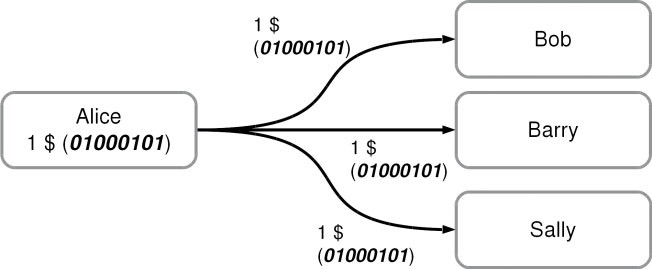
\includegraphics[width=\textwidth]{double_spending_problem.jpg}
		\caption[Double-spending problem]{Double-spending problem, da ``Understanding Bitcoin" \cite{understanding_bitcoin} figura 2.1}
		\label{fig:double-spending_img}
	\end{figure}

	\subsection{Database centralizzato}
		\begin{figure}[ht]
			\centering
			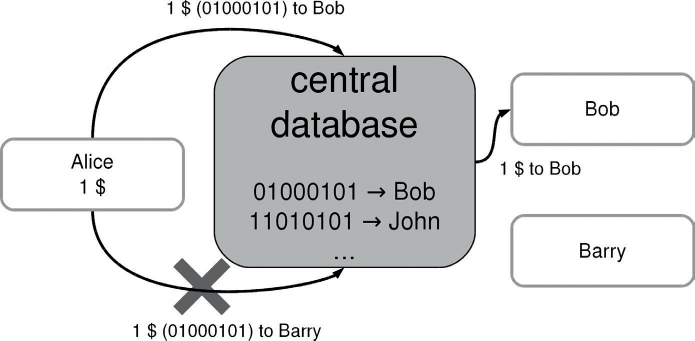
\includegraphics[width=\textwidth]{central_counterparty.png}
			\caption[Central counterparty holding a centralized database]{Central counterparty holding a centralized database, da ``Understanding Bitcoin" \cite{understanding_bitcoin} figura 2.2}
			\label{fig:central_counterparty_img}
		\end{figure}
		La soluzione contro il \emph{double-spending} finora adottata è stata l'affidamento delle transazioni economiche digitali ad un ente esterno fidato (e.g. i sistemi e-banking) che conoscesse le identità degli utenti e potesse verificarne l'effettiva disponibilità economica. È il database centrale che traccia la storia delle transazioni effettuate da ogni utente e prima di autorizzare la successiva verifica che non ci siano incongruenze. \\
		Affidarsi ad un sistema centralizzato risolve il problema, ma porta con sé una serie di criticità. \\
		Prima di tutto la necessità di \emph{trust}, fiducia, nei confronti dell'intermediario centrale: esso infatti ha libero accesso ai dati degli utenti e alla loro storia transazionale, si occupa dell'affidabilità dell'intero sistema, può autorizzare o negare transazioni e bloccare interi utenti. Si tratta di un nodo cruciale per la sicurezza del sistema, un attacco riuscito nei suoi confronti comporterebbe conseguenze disastrose. Inoltre, il database rappresenta un \emph{single point of failure}: abbattere il nodo centrale significa abbattere l'intera rete.

	\subsection{Sistemi distribuiti}
		Un'alternativa ad un sistema controllato da un intermediario centrale è rappresentata da un sistema distribuito decentralizzato. In un sistema distribuito due o più nodi collaborano per svolgere un compito prefissato in maniera trasparente all'utente, che si interfaccia con un'unica piattaforma logica. Emerge la necessità di coordinare i diversi attori: i nodi possono essere onesti e funzionare in modo corretto oppure difettosi, mal funzionanti o maliziosi. Anche se qualche nodo si rivelasse difettoso o la connessione venisse a mancare, un buon sistema distribuito dovrebbe assorbire l'imprevisto e continuare a lavorare senza problemi. La complessità di progettazione di sistemi di questo tipo non è indifferente, è stata area di ricerca fertile per molti anni e lo è tuttora. Un risultato importante è il teorema CAP, che dimostra come non possano coesistere tutte le caratteristiche desiderate in uno stesso sistema.

		\subsubsection{Teorema CAP}\label{sec:teorema_CAP}
			Altrimenti noto come Teorema di Brewer, proposto da Eric Brewer nel 1998 e dimostrato poi da Seth Gilbert e Nancy Lynch nel 2002 \cite{CAP}, il teorema CAP afferma che un qualsiasi sistema distribuito non può garantire simultaneamente le tre seguenti proprietà:
			\begin{itemize}
				\item \textbf{Coerenza (Consistency)} è la proprietà che assicura che tutti i nodi del sistema posseggono la stessa copia aggiornata dei dati;
				\item \textbf{Disponibilità (Availability)} indica che il sistema è attivo, accessibile e pronto a ricevere input e a fornire output corretti nei tempi previsti;
				\item \textbf{Tolleranza di partizione (Partition tolerance)} assicura che anche nel caso un gruppo di nodi crollasse per qualche motivo, il sistema continuerebbe ad operare correttamente.
			\end{itemize}
			\begin{figure}[ht]
				\centering
				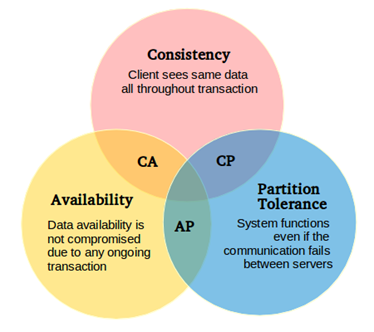
\includegraphics[width=0.7\textwidth]{cap.png}
				\caption[Teorema CAP]{Teorema CAP \cite{cap_diagram}}
				\label{fig:cap}
			\end{figure}

		\subsubsection{Problema dei Generali Bizantini}
			Si tratta di un quesito posto da Leslie Lamport (con Marshall Pease e Robert Shostak) nel 1982 \cite{BGP}, dove un gruppo di generali a capo di diverse sezioni dell'esercito bizantino sta pianificando di attaccare una città. L'unico modo a loro disposizione per comunicare è mediante messaggeri, e hanno bisogno di concordare il momento dell'attacco per vincere. Potrebbero esserci traditori tra di loro, i quali comunicherebbero messaggi discordanti per minare la riuscita dell'operazione: è quindi necessario stabilire un sistema affidabile per raggiungere il consenso sulle tempistiche di attacco. È facile l'analogia con un sistema informatico distribuito in cui i generali siano rappresentati dai nodi e i messaggeri come un'infrastruttura di rete. Una soluzione praticabile del problema dei generali bizantini in un sistema sincrono è stata proposta da Miguel Castro e Barbara Liskov in \emph{Practical Byzantine Fault Tolerance} \cite{PBFT}, mentre Bitcoin è la prima implementazione pratica con la sua soluzione basata sulla Proof-of-Work.

		\subsubsection{Algoritmi di consenso}
			La ricerca sui modi per raggiungere il consenso tra nodi di un sistema distribuito si è sviluppata molto nel periodo successivo all'introduzione di Bitcoin, pertanto sarebbe quantomeno ottimistico fornire un elenco di metodi che volesse essere esaustivo. È possibile tuttavia individuare due categorie principali di algoritmi:
			\begin{itemize}
				\item \textbf{Basati sulla fault-tolerance Bizantina}, si affidano ad un insieme di nodi che si scambiano messaggi firmati. Non richiedono impiego di risorse intensivo, sono affidabili fintanto che $N > 3F$ dove N è il numero di nodi e F è il numero di nodi malevoli;
				\item \textbf{Basati sul riconoscimento di un leader}, mettono i nodi in competizione per essere riconosciuti come leader e il nodo vincitore propone un accordo. Tipicamente richiedono un impiego di risorse considerevole come ``gara" e la sicurezza delle loro applicazioni spesso si basa proprio sulla non convenienza di un tale investimento per un attaccante.
			\end{itemize}

\section{Bitcoin}
	Il 31 ottobre del 2008, uno sconosciuto (o un gruppo) sotto lo pseudonimo di Satoshi Nakamoto annuncia la pubblicazione di un suo paper \cite{nakamoto_bitcoin} in cui presenta un nuovo sistema di moneta elettronica: Bitcoin. Non si tratta del primo esperimento di moneta elettronica, ma la notizia fa scalpore poiché Bitcoin viene presentato come completamente peer-to-peer, senza necessità di mediazione da parte di un intermediario fidato. \\
	Il sistema Bitcoin consiste, in estrema sintesi, in un registro distribuito di transazioni. Chiunque voglia usufruire del sistema per ricevere pagamenti o effettuarli deve possedere una coppia di chiavi pubblica e privata. La chiave privata serve a firmare le nuove transazioni, mentre la chiave pubblica viene diffusa e utilizzata per verificare la firma apposta sul pagamento. L'utente è identificato all'interno del registro tramite un hash della sua chiave pubblica, ovvero il suo \emph{indirizzo Bitcoin}. \\
	Nella proposta di transazione, l'utente deve dichiarare:
	\begin{itemize}
		\item l'indirizzo del destinatario;
		\item l'importo da trasferire;
		\item il riferimento alla transazione tramite cui ha ottenuto il possesso dei bitcoin che sta spendendo.
	\end{itemize}
	\begin{figure}[ht]
		\centering
		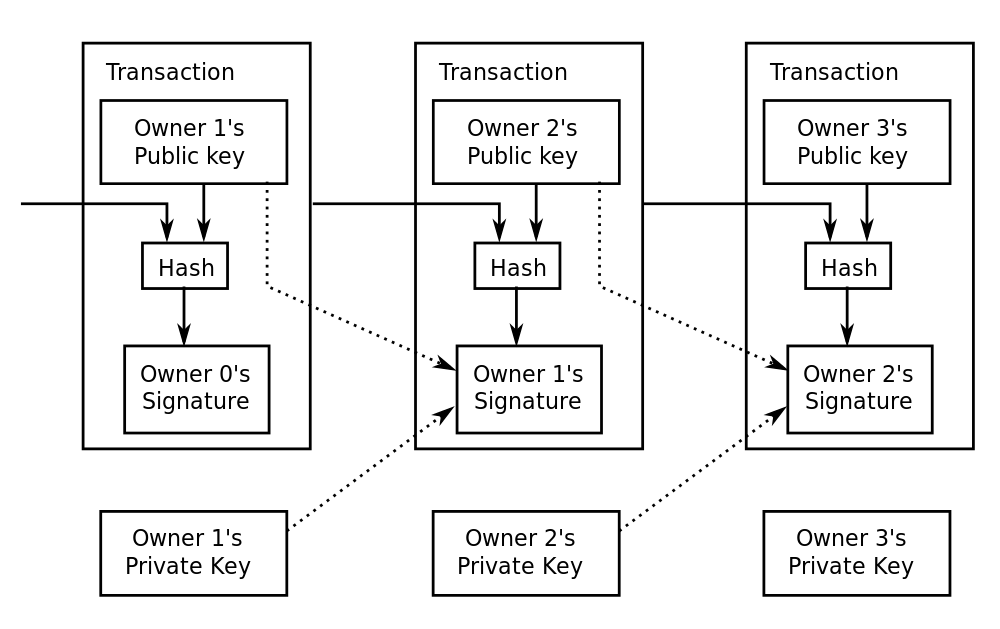
\includegraphics[width=\textwidth]{bitcoin_transaction.png}
		\caption{Struttura di una transazione}
		\label{fig:bitcoin_transaction}
	\end{figure}
	Deve inoltre fornire prova della sua identità firmando la proposta tramite la sua chiave privata.
	\subsection{Evitare il double-spending: la nascita di Blockchain}
		La crittografia asimmetrica e in particolare i concetti di firma digitale su sui si fonda il sistema descritto fino a questo punto sono ben noti da anni e largamente utilizzati molto tempo prima della nascita di Bitcoin. Non sono sufficienti però ad evitare il problema del double spending: per fare ciò è necessario assicurare l'immutabilità del registro e prevenire la creazione di transazioni non valide sfruttando la mancanza di ``accordi" tra i nodi della rete. La tecnologia adottata da Bitcoin per questo scopo è nota come \emph{Blockchain}. \\
		Il registro distribuito di Bitcoin prende la forma di una serie di ``blocchi" di transazioni legati fra di loro tramite hash crittografico: ogni blocco contiene, oltre alle transazioni che lo compongono, anche l'hash del blocco precedente permettendo quindi di individuare un ordine totale nell'insieme dei blocchi che può prendere quindi il nome di \emph{catena}. 
		\begin{figure}[ht]
			\centering
			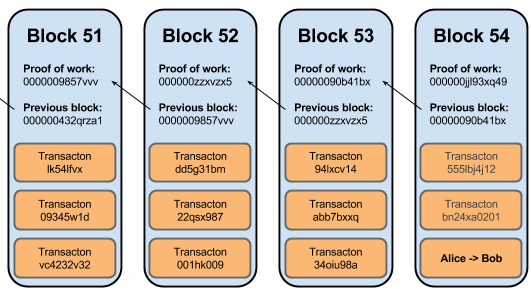
\includegraphics[width=\textwidth]{bitcoin-block-chain.png}
			\caption{Struttura a blocchi del registro}
			\label{fig:bitcoin_chain}
		\end{figure}
		\subsubsection{Consenso tramite proof-of-work}
			Rendere ordinato il registro permette di determinare in maniera univoca quale transazione sia avvenuta per prima, e quindi nel caso di doppia spesa di una particolare somma rifiutare le transazioni successive alla prima. Ciò non impedisce però ad un utente malevolo di creare una nuova catena che riassegni arbitrariamente certe somme (ad esempio modificando il destinatario di una transazione da lui effettuata) e presentarla come corretta al resto della rete. Bitcoin affronta questa eventualità rallentando la produzione dei blocchi attraverso la richiesta di una \emph{proof-of-work}. \\
			Ciascun nodo che volesse validare un nuovo blocco e proporlo al resto della rete (chiamato \emph{miner}) deve prima risolvere un problema computazionalmente molto oneroso (risolvibile solamente a forza bruta) basato su di un hash del blocco in ``lavorazione" \cite{hashcash}. In particolare, nel blocco è inserito un numero detto \emph{nonce} che deve essere determinato dal nodo proponente affinché l'hash del blocco stesso cominci con un determinato numero di 0 iniziali. Il numero di 0 richiesti influenza la difficoltà del problema: viene determinato algoritmicamente sul tempo medio di creazione degli ultimi blocchi e ciò fa in modo che il tempo necessario si assesti non sotto i 10 minuti. \\
			\begin{figure}[ht]
				\centering
				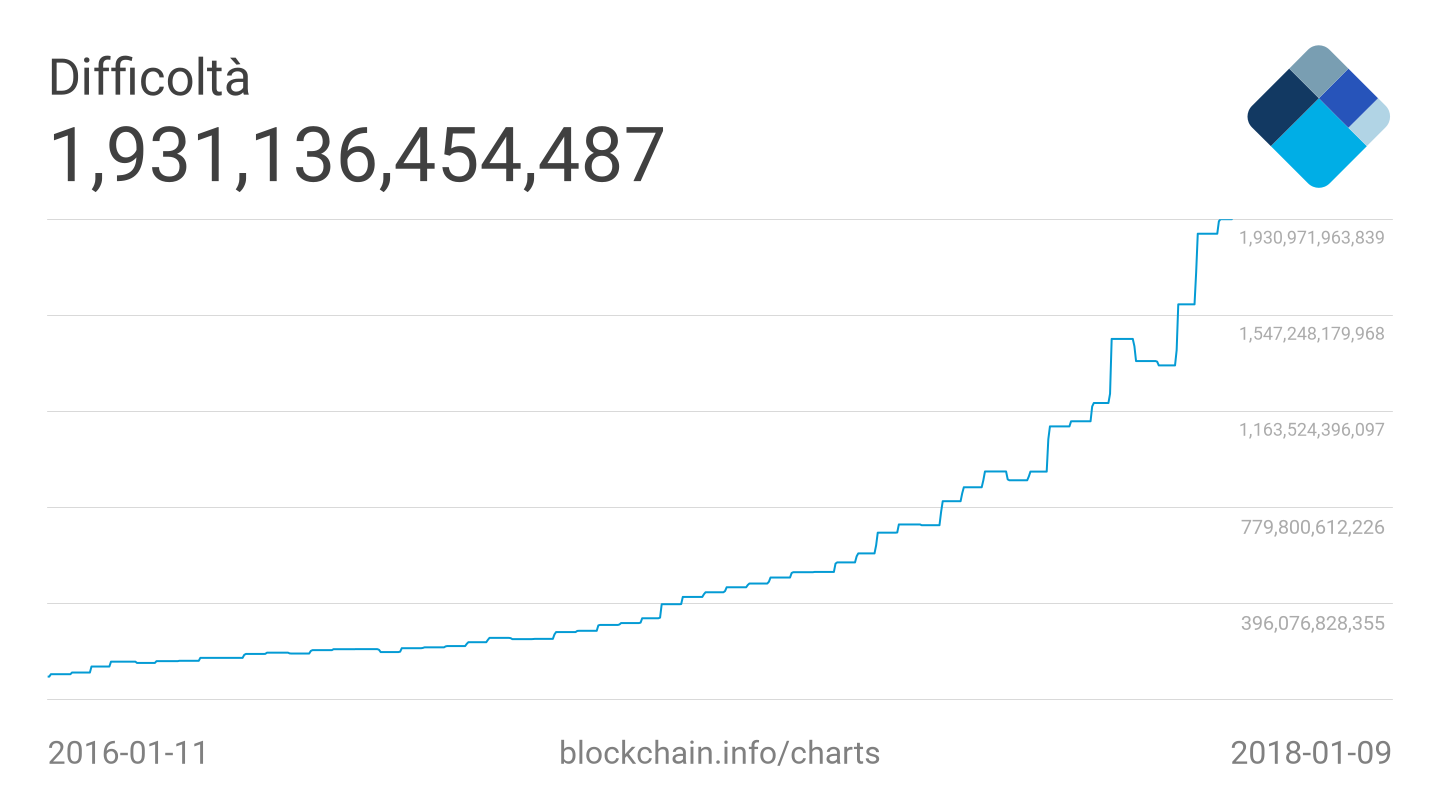
\includegraphics[width=\textwidth]{difficulty.png}
				\caption{Difficoltà di creazione di un nuovo blocco}
				\label{fig:bitcoin_difficulty}
			\end{figure}
			Questo \emph{sforzo} necessario da parte dei miner fa sì che un nodo malevolo che volesse creare nuova catena alterata dovrebbe ricalcolare la soluzione a tutti i problemi matematici relativi a tutti i blocchi successivi a quello alterato. Dal momento che la rete accetta come corretta solamente la catena più lunga, tale attaccante dovrebbe validare i blocchi più velocemente del resto della rete, per poter ad un certo punto superare la lunghezza della blockchain ``ufficiale" e veder riuscire il suo attacco.
		
		\subsubsection{Il guadagno dei miner}
			L'introduzione di un simile onere pesa tanto su di un ipotetico attaccante quanto sul resto della rete: per fornire un adeguato incentivo per il mantenimento della rete, la prima transazione di ogni blocco è \emph{autorizzata a creare nuovi bitcoin} in favore del miner che l'ha validato. Questo è l'unico modo in cui nuovi bitcoin possono essere creati, e l'ammontare di questa ricompensa è anch'esso algoritmicamente determinato. La presenza di questa ricompensa fa in modo che sia più profittevole, da parte di un nodo con sufficiente potenza di calcolo da impensierire la stabilità della rete, investire queste risorse nel mantenimento della rete stessa svolgendo il ruolo di miner invece che in attacchi come quello descritto sopra.
			\paragraph{Offerta anelastica e scenario futuro} ~ \\
				È necessario un piccolo appunto sulla possibile evoluzione di questo equilibrio: la ricompensa per la validazione di un blocco è infatti destinata a ridursi con il tempo. L'algoritmo prevede infatti che questa venga dimezzata ogni circa 4 anni fino a raggiungere una quantità di bitcoin immessi di circa 21 milioni.
				\begin{figure}[ht]
					\centering
					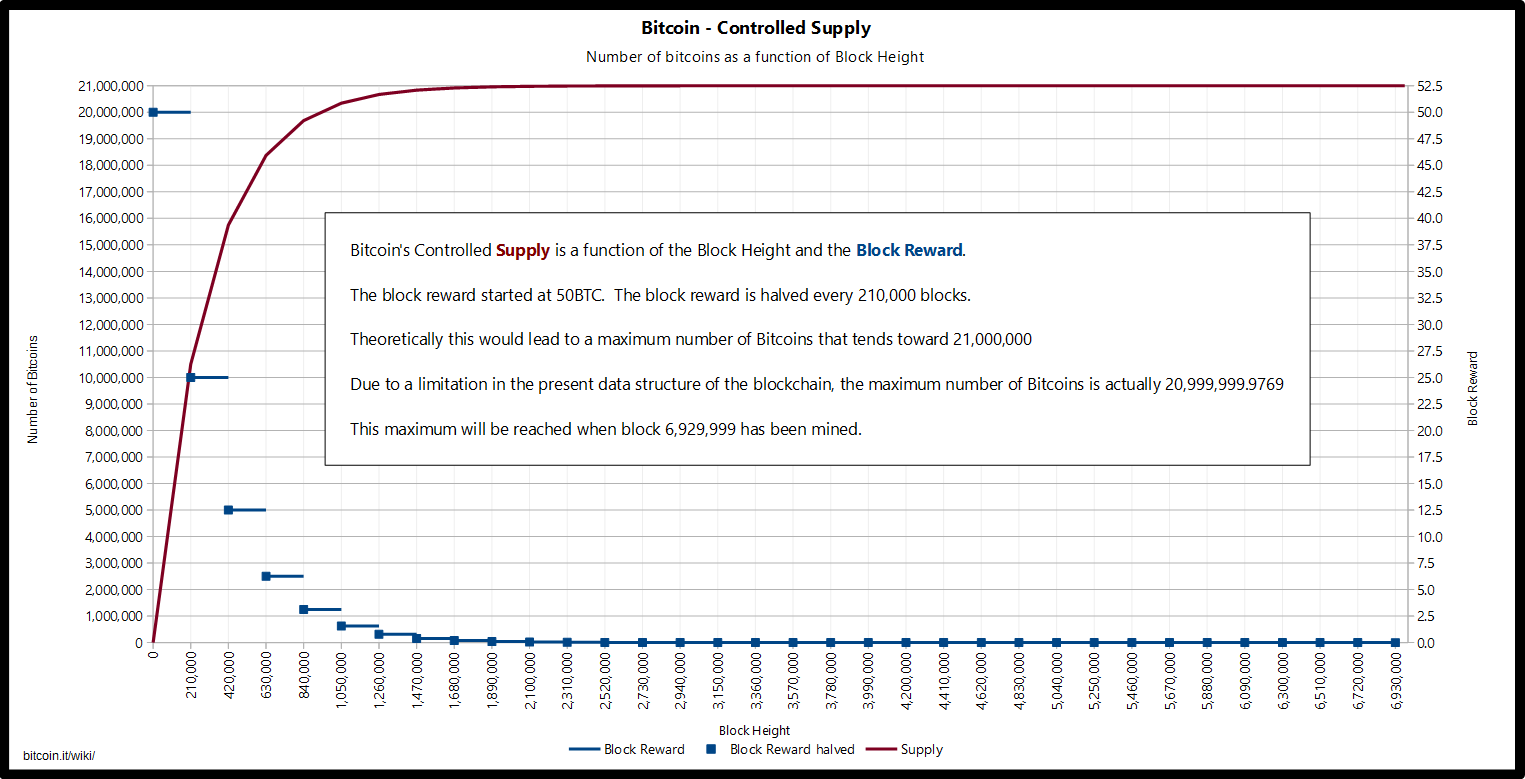
\includegraphics[width=\textwidth]{bitcoin_supply.png}
					\caption{Emissione fissata di bitcoin}
					\label{fig:bitcoin_supply}
				\end{figure}
				L'ultima frazione di bitcoin generata sarà creata nel 2141: a quel punto verrà meno, apparentemente, l'incentivo al mining ``onesto". Nonostante questo possa sembrare uno scenario remoto per via della data ancora sufficientemente distante nel tempo, il problema è più attuale di quanto sembri per via degli enormi costi delle attrezzature per il mining. La competizione in quest'ambito si è accesa e ha dato il via ad una corsa continua per accumulare la maggior potenza di calcolo possibile, alzando moltissimo la quantità di risorse necessarie in termini di hardware ed energia. Il momento in cui questi costi supereranno il valore della ricompensa è quindi molto più vicino della data di emissione dell'ultimo bitcoin. \\
				A mantenere l'equilibrio c'è la possibilità da parte dei nodi di includere una tassa volontaria a destinatario libero all'interno delle proprie transazioni. Il miner che include la transazione all'interno del blocco in validazione imposta se stesso come destinatario di questa offerta che quindi va a partecipare all'incentivo economico necessario per il mantenimento della rete.